%!TEX encoding = UTF-8 Unicode
%!TEX program = xelatex
%!BIB program = bibtex

% ============================================================
% 中国原子能科学研究院（CIAE）学位论文 LaTeX 模板
% 使用前请阅读各章节文件中的注释说明
% 编译方式：xelatex -> bibtex -> xelatex -> xelatex
% ============================================================

\documentclass[doctor,chinese,print]{ustcthesis}
% 学位类型选项：master（硕士）| doctor（博士），选择后页眉自动切换
% 语言选项：chinese（中文）
\usepackage{ustcextra}
% subcaption 已在 ustcthesis.cls 中加载，此处无需重复
\graphicspath{{figures/}}   % 图片搜索路径，建议将所有图片放于 figures/ 目录下

% 参考文献格式：gbt7714-numerical（顺序编码制，推荐）
%               ustcauthoryear（著者-出版年制）
\newcommand{\upcite}[1]{\textsuperscript{\textsuperscript{\cite{#1}}}}  % 上标引用命令

% ============================================================
% 封面信息填写区（请替换尖括号内的占位符）
% ============================================================

\classnum{O571.6}               % 分类号（中图分类号）
\secretlevel{非密}              % 密级：非密|内部|秘密|机密
\title{基于XXXX的研究\\换行测试}          % 论文中文题目
\author{张~三~三}               % 作者姓名（姓名间用~分隔以调整间距）
\major{粒子物理与原子核物理}     % 学科专业
\advisor{李四}              % 导师姓名
\depart{研究员}                 % 导师职称
\coadvisor{王五}            % 副导师姓名（如有，取消注释）
\codepart{副研究员}         % 副导师职称（如有，取消注释）
% \secrettext{机密\quad 小于等于20年}   % 密级：内部|秘密|机密，不涉密则注释本行
\submitdate{2025.5}             % 论文提交日期
\defensedate{2025.5}            % 论文答辩日期
\grantdate{2025.7}              % 学位授予日期
\chairman{张六六}               % 答辩委员会主席
\reviewer{赵七、吴九九、刘十}         % 评阅人
\coverdate{2025年5月}           % 封面底部日期

% 英文封面信息（如需英文封面，取消注释并填写）
% \entitle{Research on XXX Based on XXXX}
% \enauthor{Zhang Sansan}
% \enmajor{Particle Physics and Nuclear Physics}
% \enadvisor{Prof. Li Sisi}
% \ensubmitdate{June, 202X}
% \ensecrettext{Confidential\quad Less than or equal to 20 years}

\begin{document}

\maketitle

% ============================================================
% 论文结构说明：
%   frontmatter：中文摘要、英文摘要、目录、图目录、表目录、符号说明
%   mainmatter ：正文各章节、参考文献
%   appendix   ：附录
%   backmatter ：致谢、发表论文列表
% ============================================================

\frontmatter
\begin{abstract}

本模板是面向中国原子能科学研究院（CIAE）硕士、博士研究生的学位论文 \LaTeX{} 排版模板，
基于中国科学技术大学论文模板（ustcthesis）修改而来，
在保留原模板完善排版功能的基础上，针对原子能院的封面格式与论文规范进行了适配。

本模板的目标是将论文格式与论文内容分离，
使作者专注于论文内容的写作，而无需过多关注排版细节。
模板已预设符合学院要求的页面尺寸、字体字号、页眉页脚、参考文献格式等，
开箱即用，按照各章注释提示填写内容即可。

% -------------------------------------------------------
% 摘要写作说明：
%   1. 中文摘要一般为 500 字左右（硕士），博士可适当增加。
%   2. 摘要应概括研究目的、方法、主要结果和结论，不宜涉及推导过程。
%   3. 避免出现参考文献、图表编号等。
%   4. 关键词 3～8 个，各词之间用 、 分隔。
% -------------------------------------------------------

\keywords{中国原子能科学研究院、学位论文、 \LaTeX{}、模板、排版}
\end{abstract}

\begin{enabstract}

This template is a \LaTeX{} dissertation typesetting template for master's and doctoral
students at the China Institute of Atomic Energy (CIAE).
It is adapted from the ustcthesis template of the University of Science and Technology of China,
with modifications to cover formats and thesis specifications tailored to CIAE requirements.

The goal of this template is to separate document formatting from content,
allowing authors to focus on writing without worrying about typesetting details.
Page layout, fonts, headers and footers, and reference styles are all preset
to meet institutional requirements.

% -------------------------------------------------------
% English abstract notes:
%   1. The English abstract should match the Chinese version in content.
%   2. Aim for around 300 words for a master's thesis.
%   3. Use the past tense when describing methods and results.
%   4. Keywords should correspond to the Chinese keywords.
% -------------------------------------------------------

\enkeywords{China Institute of Atomic Energy, Dissertation, \LaTeX{} Template, Typesetting}
\end{enabstract}
        % 中英文摘要
{
\linespread{1.25}\selectfont     % 目录局部行距
\tableofcontents                 % 目录
\listoffigures                   % 图目录（如无图，可注释）
\listoftables                    % 表目录（如无表，可注释）
}
% \listofalgorithms              % 算法索引（如不需要，保持注释）
% \input{chapters/notation}      % 符号说明（如不需要，保持注释）

% 自定义定理环境（按需增减）
\newtheorem{proof_idea}{证明思路}
\newtheorem{thm}{定理}

\mainmatter

%%% Local Variables:
%%% mode: latex
%%% TeX-master: t
%%% End:

% ============================================================
% 第一章：快速开始
% 本章介绍模板的基本使用方法，适合从未接触过 LaTeX 的读者。
% 写正式论文时，请将本章内容替换为你的绪论。
% ============================================================

\chapter{快速开始}\label{chap:quickstart}

\section{模板背景与优势}

本模板为中国原子能科学研究院（CIAE）学位论文 \LaTeX{} 排版模板，
适用于硕士与博士研究生撰写学位论文。
模板基于中国科学技术大学的 ustcthesis 文档类，
针对院内格式规范对封面样式、页眉页脚、参考文献格式进行了修改。

使用 \LaTeX{} 撰写论文的主要优势：

\begin{compactitem}
    \item \textbf{格式与内容分离}：模板自动处理所有排版格式，作者只需专注于写作内容。
    \item \textbf{公式排版精美}：数学公式是 \LaTeX{} 的强项，核物理公式、矩阵、积分均可高质量输出。
    \item \textbf{参考文献自动化}：添加文献到 \texttt{.bib} 文件后，编号和格式全部自动生成。
    \item \textbf{编号自动更新}：插入或删除图、表、章节后，所有引用编号自动重新计算。
    \item \textbf{版本管理友好}：纯文本文件，可用 Git 进行版本控制，方便与导师协作修改。
\end{compactitem}

\section{模板文件结构}

使用本模板时，你主要需要接触以下文件：

\begin{compactitem}
    \item \texttt{main.tex}：\textbf{主文件}，填写封面信息，控制章节组织。每次修改后需重新编译。
    \item \texttt{chapters/abstract.tex}：填写中英文摘要和关键词。
    \item \texttt{chapters/chap01.tex} 至 \texttt{chap0X.tex}：论文各章正文，在这里写你的内容。
    \item \texttt{bib/refs.bib}：参考文献数据库，在这里添加所有参考文献。
    \item \texttt{figures/}：存放论文中的图片（支持 \texttt{.pdf}、\texttt{.eps}、\texttt{.png}、\texttt{.jpg}）。
    \item \texttt{chapters/acknowledgements.tex}：致谢。
    \item \texttt{chapters/publications.tex}：攻读学位期间发表的论文列表。
\end{compactitem}

以下文件定义模板格式，\textbf{一般不需要修改}：

\begin{compactitem}
    \item \texttt{ustcthesis.cls}：文档类，定义页面、字体、标题、页眉页脚等全部格式。
    \item \texttt{ustcextra.sty}：扩展宏包，提供定理、代码、算法等环境。
    \item \texttt{gbt7714-numerical.bst}：参考文献样式（国标 GB/T 7714 顺序编码制）。
\end{compactitem}

\section{填写封面信息}

打开 \texttt{main.tex}，找到封面信息填写区，修改以下命令：

\begin{compactitem}
    \item \verb|\classnum{...}|：中图分类号，如 \verb|\classnum{O571.6}|。
    \item \verb|\secretlevel{...}|：密级，填写"非密"、"内部"、"秘密"或"机密"之一，如 \verb|\secretlevel{非密}|。
    \item \verb|\title{...}|：论文中文题目，不超过35个汉字。
    \item \verb|\author{...}|：作者姓名。姓名之间用 \verb|~| 分隔可调整间距，如 \verb|\author{张~三}|。
    \item \verb|\major{...}|：学科专业名称，如"粒子物理与原子核物理"。
    \item \verb|\advisor{...}|：导师姓名。
    \item \verb|\depart{...}|：导师职称，如"研究员"。
\end{compactitem}

如需英文封面，取消以下几行注释并填写：
\begin{verbatim}
\entitle{Research on XXX Based on XXXX}
\enauthor{Zhang San}
\enmajor{Particle Physics and Nuclear Physics}
\enadvisor{Prof. Li Si}
\end{verbatim}

\subsection{切换学位类型}

在 \texttt{main.tex} 第一行修改文档类选项：

\begin{verbatim}
% 硕士论文（默认）
\documentclass[master,chinese,pdf,AutoFakeFont=true]{ustcthesis}

% 博士论文
\documentclass[doctor,chinese,pdf,AutoFakeFont=true]{ustcthesis}

% 打印版（双面打印，链接为黑色）
\documentclass[master,chinese,print,AutoFakeFont=true]{ustcthesis}
\end{verbatim}

\section{如何编译}

本模板已在以下环境测试通过：
\begin{compactitem}
    \item \textbf{Windows + TeX Live 2023 + VS Code + LaTeX Workshop}
    \item \textbf{WSL Ubuntu + TeX Live}（支持 \texttt{make}）
\end{compactitem}

\LaTeX{} 需要"编译"才能生成 PDF。本模板需要按顺序运行4步：

\begin{verbatim}
xelatex main   % 第一遍：生成辅助文件
bibtex main    % 处理参考文献
xelatex main   % 第二遍：插入参考文献
xelatex main   % 第三遍：更新所有编号
\end{verbatim}

\textbf{必须运行4次}才能保证目录、参考文献编号、交叉引用全部正确。

\subsection{使用 VS Code + LaTeX Workshop（推荐）}

\begin{compactenum}
    \item 安装 TeX Live（完整版），安装 VS Code 及 LaTeX Workshop 插件。
    \item 用 VS Code 打开模板根目录，打开 \texttt{main.tex}。
    \item 按 \texttt{Ctrl+Alt+B}，在弹出菜单中选择 Recipe：
          \textbf{xelatex → bibtex → xelatex → xelatex}。
    \item 编译完成后，按 \texttt{Ctrl+Alt+V} 预览 PDF。
\end{compactenum}

\subsection{使用 latexmk 自动编译}

模板根目录下的 \texttt{.latexmkrc} 文件配置了 \texttt{latexmk} 的编译规则，
使其自动以 \texttt{xelatex} 引擎完成完整的编译流程。
在终端中执行：

\begin{verbatim}
latexmk main
\end{verbatim}

\textbf{注意：\texttt{.latexmkrc} 文件不能删除。}
若缺少该文件，\texttt{latexmk} 将默认使用 \texttt{latex} 引擎，
导致中文无法正确编译（乱码或报错）。

\section{添加新章节}

如需增加章节：

\begin{compactenum}
    \item 在 \texttt{chapters/} 目录下新建文件，如 \texttt{chap07.tex}，内容结构如下：
\begin{verbatim}
\chapter{你的章节标题}\label{chap:标识符}

\section{第一节}
正文内容……

\section{本章小结}
本章介绍了……
\end{verbatim}
    \item 在 \texttt{main.tex} 的 \verb|\mainmatter| 区域添加一行：
\begin{verbatim}
\input{chapters/chap07}
\end{verbatim}
\end{compactenum}

\textbf{命名建议}：\verb|\label| 中的标识符用英文，如 \verb|chap:theory|、\verb|chap:experiment|，
以便后续用 \verb|\ref{chap:theory}| 引用章节编号。

\section{本章小结}

本章介绍了模板的背景、文件结构、封面信息填写、编译方法及章节添加方式。
第~\ref{chap:typesetting}~章将介绍正文排版的基本用法，
包括段落书写、标题层级、列表和交叉引用。
   % 第一章：快速开始（模板使用说明，正式论文请替换为绪论）
%%% Local Variables:
%%% mode: latex
%%% TeX-master: t
%%% End:

% ============================================================
% 第二章：文字与段落排版
% 本章介绍 LaTeX 基础排版：段落、标题、列表、引用和特殊字符。
% ============================================================

\chapter{文字与段落排版}\label{chap:typesetting}

\section{段落基础}

在 \LaTeX{} 中，\textbf{空一行}表示新段落（即按两次回车），
新段落会自动首行缩进2个汉字宽度，符合本院格式规范。

\textbf{注意事项：}

\begin{compactitem}
    \item 单次换行（按一次回车）在 \LaTeX{} 中\textbf{不会}产生换行效果，只是源码中的排版习惯。
    \item 不要使用 \verb|\\| 强制换行来分隔段落，这会破坏首行缩进。
    \item 中文之间的空格会被 \LaTeX{} 自动忽略，中英文之间会自动添加适当间距。
    \item 多个连续空格等同于一个空格。
\end{compactitem}

示例：下面两段文字在源码中用空行分隔，排版后自动产生段落缩进。

这是第一段的内容，介绍了实验的背景和意义。在实际论文中，这里应该是完整的学术内容。

这是第二段的内容，继续论述相关问题。段落间无需手动添加缩进，模板已自动配置。

\section{字体样式}

常用字体命令：

\begin{compactitem}
    \item \verb|\textbf{文字}| → \textbf{加粗文字}（黑体效果）
    \item \verb|\textit{text}| → \textit{斜体文字}（仅对英文有明显效果）
    \item \verb|\underline{文字}| → \underline{下划线文字}
    \item \verb|\texttt{text}| → \texttt{等宽字体}（用于代码、文件名）
    \item \verb|\emph{文字}| → \emph{强调文字}（英文斜体，中文加粗）
\end{compactitem}

\textbf{建议}：论文正文中尽量少用字体变化，过多装饰会影响阅读专注度。

\section{标题层级}

本模板支持三级正文标题，对应格式已由模板自动设定：

\begin{compactitem}
    \item \verb|\section{标题}|：一级标题（节），黑体四号，顶格
    \item \verb|\subsection{标题}|：二级标题（条），黑体小四号，顶格
    \item \verb|\subsubsection{标题}|：三级标题，黑体小四号
\end{compactitem}

格式规范要求：\textbf{论文中一般不出现四级标题}（即不使用 \verb|\subsubsection| 过多层级）。

每个标题后面应紧跟 \verb|\label{sec:标识符}| 以便后续交叉引用：

\begin{verbatim}
\section{实验方法}\label{sec:method}
\subsection{探测器设置}\label{sec:detector}
\end{verbatim}

\subsection{标题引用示例}

上一章第~\ref{chap:quickstart}~章介绍了快速开始的方法，
本章第~\ref{sec:crossref}~节将介绍交叉引用的具体写法。

\section{列表环境}

\LaTeX{} 提供两种主要列表环境。本模板通过 \texttt{ustcextra.sty} 提供了紧凑版本，
段落间距更小，更适合论文排版。

\subsection{无序列表}

使用 \texttt{compactitem} 环境（推荐，间距紧凑）：

\begin{verbatim}
\begin{compactitem}
    \item 第一条内容
    \item 第二条内容
    \item 第三条内容
\end{compactitem}
\end{verbatim}

效果如下：
\begin{compactitem}
    \item 能量分辨率优于 1\%
    \item 时间分辨率优于 200 ps
    \item 探测效率大于 95\%
\end{compactitem}

\subsection{有序列表}

使用 \texttt{compactenum} 环境：

\begin{verbatim}
\begin{compactenum}
    \item 第一步：初始化参数
    \item 第二步：运行模拟
    \item 第三步：分析结果
\end{compactenum}
\end{verbatim}

效果如下：
\begin{compactenum}
    \item 第一步：初始化参数
    \item 第二步：运行模拟
    \item 第三步：分析结果
\end{compactenum}

列表可以嵌套，但建议不超过两层，以保持可读性。

\section{交叉引用}\label{sec:crossref}

交叉引用是 \LaTeX{} 的重要功能，可以自动引用章节、图、表、公式的编号，
修改论文内容时编号自动更新，无需手动维护。

\subsection{基本用法}

\begin{compactenum}
    \item 在需要被引用的位置添加标签：\verb|\label{标识符}|
    \item 在引用处使用：\verb|\ref{标识符}|（显示编号）
\end{compactenum}

推荐的标识符命名规范：

\begin{compactitem}
    \item 章节：\verb|chap:introduction|、\verb|sec:method|
    \item 图：\verb|fig:detector|、\verb|fig:result|
    \item 表：\verb|tab:parameters|、\verb|tab:results|
    \item 公式：\verb|eq:schrodinger|、\verb|eq:cross_section|
\end{compactitem}

引用示例：

\begin{verbatim}
如图~\ref{fig:detector}~所示，探测器由三层组成。
表~\ref{tab:parameters}~列出了实验参数。
由公式~(\ref{eq:cross_section})~可得截面值。
详见第~\ref{chap:experiment}~章。
\end{verbatim}

\textbf{注意}：在 \verb|\ref{}| 两侧使用 \verb|~|（波浪线）表示不可断行空格，
避免"图"字与编号被分到两行。

\section{特殊字符的输入}

以下字符在 \LaTeX{} 中有特殊含义，直接输入会报错，需要转义：

\begin{table}[H]
\centering
\bicaption{特殊字符输入方法}{Special character input methods}
\begin{tabular}{cll}
\hline
字符 & 含义 & 输入方式 \\
\hline
\texttt{\%} & 注释符 & \verb|\%| \\
\texttt{\$} & 公式符 & \verb|\$| \\
\texttt{\&} & 表格列分隔 & \verb|\&| \\
\texttt{\#} & 宏参数 & \verb|\#| \\
\texttt{\_} & 下标 & \verb|\_| \\
\texttt{\{} \texttt{\}} & 分组 & \verb|\{| \verb|\}| \\
\texttt{\^{}} & 上标 & \verb|\^{}| \\
\texttt{\~{}} & 不断行空格 & \verb|\~{}| \\
\hline
\end{tabular}
\end{table}

其他常用输入：
\begin{compactitem}
    \item 省略号：\verb|\ldots| → \ldots （不要用三个英文句号）
    \item 破折号：\verb|——|（直接输入中文破折号）或 \verb|---| → ---
    \item 连字符：\verb|-|（单个减号，用于复合词，如 time-of-flight）
    \item 数字范围：\verb|--| → 1--10（长短介于 - 和 ---之间）
\end{compactitem}

\section{本章小结}

本章介绍了段落书写规范、字体样式、标题层级、列表环境、
交叉引用和特殊字符的使用方法。
第~\ref{chap:math}~章将介绍数学公式和定理环境的写法，
这是核物理论文中最常用的排版功能之一。
   % 第二章：文字与段落排版
%%% Local Variables:
%%% mode: latex
%%% TeX-master: t
%%% End:

% ============================================================
% 第三章：数学公式与定理
% 本章介绍 LaTeX 数学排版，包括公式、符号速查和定理环境。
% ============================================================

\chapter{数学公式与定理}\label{chap:math}

\section{行内公式}

行内公式嵌入在正文中，用一对美元符号 \verb|$ $| 包围：

\begin{verbatim}
质子的静止质量为 $m_p = 938.3$ MeV/$c^2$。
\end{verbatim}

效果：质子的静止质量为 $m_p = 938.3$ MeV/$c^2$。

常用行内公式写法：
\begin{compactitem}
    \item 下标：\verb|$a_i$| → $a_i$，上标：\verb|$E^2$| → $E^2$
    \item 分数（行内）：\verb|$m/c^2$| → $m/c^2$（行内分数建议用斜线形式）
    \item 希腊字母：\verb|$\alpha, \beta, \gamma$| → $\alpha, \beta, \gamma$
    \item 向量（粗体）：\verb|$\mathbf{p}$| → $\mathbf{p}$
\end{compactitem}

\section{行间公式}

行间公式独立成行，用 \texttt{equation} 环境，自动按章节编号：

\begin{verbatim}
\begin{equation}
    E = mc^2
    \label{eq:einstein}
\end{equation}
\end{verbatim}

\begin{equation}
    E = mc^2
    \label{eq:einstein}
\end{equation}

由式~(\ref{eq:einstein})~可知，质能等价。

更复杂的示例——薛定谔方程：
\begin{equation}
    i\hbar \frac{\partial}{\partial t} \Psi(\mathbf{r}, t)
    = \left[ -\frac{\hbar^2}{2m} \nabla^2 + V(\mathbf{r}, t) \right] \Psi(\mathbf{r}, t)
    \label{eq:schrodinger}
\end{equation}

\textbf{格式规范}：按格式要求，公式序号右端对齐，
\texttt{equation} 环境已自动处理。
公式中第一次出现的物理量符号应在公式后用"式中"段落注释。

\subsection{公式后的符号注释}

格式规范要求对公式中的物理量进行说明，写法如下：

\begin{verbatim}
\begin{equation}
    \sigma = \frac{I_0 - I}{I_0 N t}
    \label{eq:cross_section}
\end{equation}

式中：$\sigma$——反应截面（cm$^2$）；\\
\phantom{式中：}$I_0$——入射粒子数；\\
\phantom{式中：}$I$——出射粒子数；\\
\phantom{式中：}$N$——靶核数密度（cm$^{-3}$）；\\
\phantom{式中：}$t$——靶厚（cm）。
\end{verbatim}

\begin{equation}
    \sigma = \frac{I_0 - I}{I_0 N t}
    \label{eq:cross_section}
\end{equation}

式中：$\sigma$——反应截面（cm$^2$）；\\
\phantom{式中：}$I_0$——入射粒子数；\\
\phantom{式中：}$I$——出射粒子数。

\section{多行公式}

当公式较长需要换行，或需要对齐多个等式时，使用 \texttt{align} 环境：

\begin{verbatim}
\begin{align}
    Q &= (M_A + M_a - M_B - M_b)c^2  \label{eq:q_value} \\
      &= T_B + T_b - T_a              \label{eq:q_kinetic}
\end{align}
\end{verbatim}

\begin{align}
    Q &= (M_A + M_a - M_B - M_b)c^2  \label{eq:q_value} \\
      &= T_B + T_b - T_a              \label{eq:q_kinetic}
\end{align}

\verb|&| 表示对齐位置，\verb|\\| 换行。每行都有独立编号。

如果不需要某行编号，在该行末尾加 \verb|\nonumber|：
\begin{verbatim}
\begin{align}
    f(x) &= x^2 + 2x + 1  \nonumber \\
         &= (x+1)^2       \label{eq:factor}
\end{align}
\end{verbatim}

\section{矩阵}

\begin{verbatim}
\begin{equation}
    \mathbf{A} = \begin{pmatrix}
        a_{11} & a_{12} & \cdots & a_{1n} \\
        a_{21} & a_{22} & \cdots & a_{2n} \\
        \vdots & \vdots & \ddots & \vdots \\
        a_{m1} & a_{m2} & \cdots & a_{mn}
    \end{pmatrix}
\end{equation}
\end{verbatim}

\begin{equation}
    \mathbf{A} = \begin{pmatrix}
        a_{11} & a_{12} & \cdots & a_{1n} \\
        a_{21} & a_{22} & \cdots & a_{2n} \\
        \vdots & \vdots & \ddots & \vdots \\
        a_{m1} & a_{m2} & \cdots & a_{mn}
    \end{pmatrix}
\end{equation}

矩阵括号类型：
\begin{compactitem}
    \item \texttt{pmatrix}：圆括号 $(\,)$
    \item \texttt{bmatrix}：方括号 $[\,]$
    \item \texttt{vmatrix}：竖线（行列式）$|\,|$
    \item \texttt{Bmatrix}：花括号 $\{\,\}$
\end{compactitem}

\section{常用数学符号速查}

\subsection{希腊字母}

\begin{table}[H]
\centering
\bicaption{常用希腊字母}{Common Greek letters}
\begin{tabular}{llll|llll}
\hline
命令 & 符号 & 命令 & 符号 & 命令 & 符号 & 命令 & 符号 \\
\hline
\verb|\alpha|   & $\alpha$   & \verb|\Alpha|   & $A$       & \verb|\beta|    & $\beta$    & \verb|\gamma|   & $\gamma$ \\
\verb|\delta|   & $\delta$   & \verb|\Delta|   & $\Delta$  & \verb|\epsilon| & $\epsilon$ & \verb|\theta|   & $\theta$ \\
\verb|\lambda|  & $\lambda$  & \verb|\Lambda|  & $\Lambda$ & \verb|\mu|      & $\mu$      & \verb|\nu|      & $\nu$ \\
\verb|\pi|      & $\pi$      & \verb|\Pi|      & $\Pi$     & \verb|\sigma|   & $\sigma$   & \verb|\Sigma|   & $\Sigma$ \\
\verb|\phi|     & $\phi$     & \verb|\Phi|     & $\Phi$    & \verb|\psi|     & $\psi$     & \verb|\Psi|     & $\Psi$ \\
\verb|\omega|   & $\omega$   & \verb|\Omega|   & $\Omega$  & \verb|\eta|     & $\eta$     & \verb|\xi|      & $\xi$ \\
\hline
\end{tabular}
\end{table}

\subsection{常用运算符}

\begin{compactitem}
    \item 积分：\verb|\int_0^\infty f(x)dx| → $\int_0^\infty f(x)dx$
    \item 求和：\verb|\sum_{i=1}^{n} a_i| → $\sum_{i=1}^{n} a_i$
    \item 乘积：\verb|\prod_{i=1}^{n}| → $\prod_{i=1}^{n}$
    \item 分数：\verb|\frac{分子}{分母}| → $\frac{a+b}{c}$
    \item 根号：\verb|\sqrt{x}|, \verb|\sqrt[3]{x}| → $\sqrt{x}$, $\sqrt[3]{x}$
    \item 偏微分：\verb|\partial| → $\partial$
    \item 约等于：\verb|\approx| → $\approx$；正比于：\verb|\propto| → $\propto$
    \item 向量算符：\verb|\nabla| → $\nabla$；\verb|\hbar| → $\hbar$
\end{compactitem}

\section{定理、引理与证明环境}

模板在 \texttt{ustcextra.sty} 中预定义了以下环境：

\begin{verbatim}
定理:     \begin{theorem}...\end{theorem}
引理:     \begin{lemma}...\end{lemma}
推论:     \begin{corollary}...\end{corollary}
定义:     \begin{definition}...\end{definition}
命题:     \begin{proposition}...\end{proposition}
注:       \begin{remark}...\end{remark}
证明:     \begin{proof}...\end{proof}
\end{verbatim}

示例——一个简单的定理及其证明：

\begin{theorem}
    对于任意实数 $a$ 和 $b$，有 $(a+b)^2 = a^2 + 2ab + b^2$。
\end{theorem}

\begin{proof}
    展开左边：$(a+b)^2 = (a+b)(a+b) = a^2 + ab + ba + b^2 = a^2 + 2ab + b^2$，
    故等式成立。
\end{proof}

定理类环境按章节自动编号。在 \texttt{main.tex} 中可以用 \verb|\newtheorem| 自定义新的定理类环境。

\section{本章小结}

本章介绍了行内公式、行间公式、多行公式对齐、矩阵写法、
常用数学符号以及定理环境的使用方法。
第~\ref{chap:floats}~章将介绍图片和表格的插入与排版。
   % 第三章：数学公式与定理
%%% Local Variables:
%%% mode: latex
%%% TeX-master: t
%%% End:

% ============================================================
% 第四章：图片与表格
% 本章介绍图片插入、表格制作和浮动体的使用方法。
% ============================================================

\chapter{图片与表格}\label{chap:floats}

\section{插入图片}

\subsection{基本用法}

图片使用 \texttt{figure} 浮动环境，\LaTeX{} 会自动选择最合适的位置放置：

\begin{verbatim}
\begin{figure}[htbp]
    \centering
    \includegraphics[width=0.6\textwidth]{你的图片文件名}
    \bicaption{中文图题}{English caption}
    \label{fig:示例}
\end{figure}
\end{verbatim}

实际效果如图~\ref{fig:ion}~所示：

\begin{figure}[htbp]
    \centering
    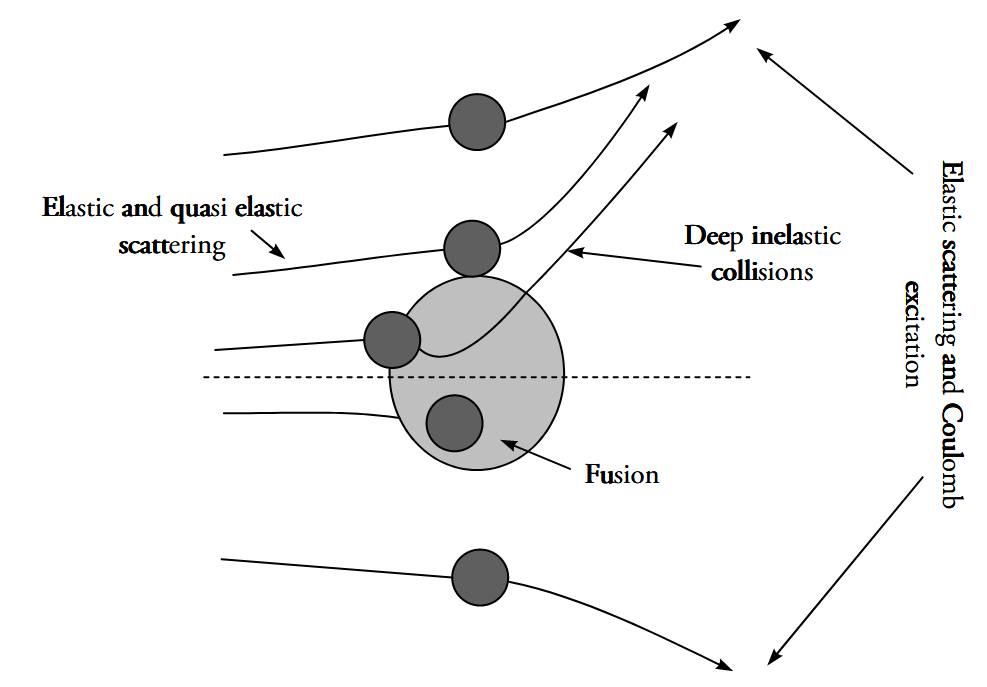
\includegraphics[width=0.6\textwidth]{ion}
    \bicaption{离子示意图}{Schematic diagram of ions}
    \label{fig:ion}
\end{figure}

如图~\ref{fig:lcn}~所示：

\begin{figure}[htbp]
    \centering
    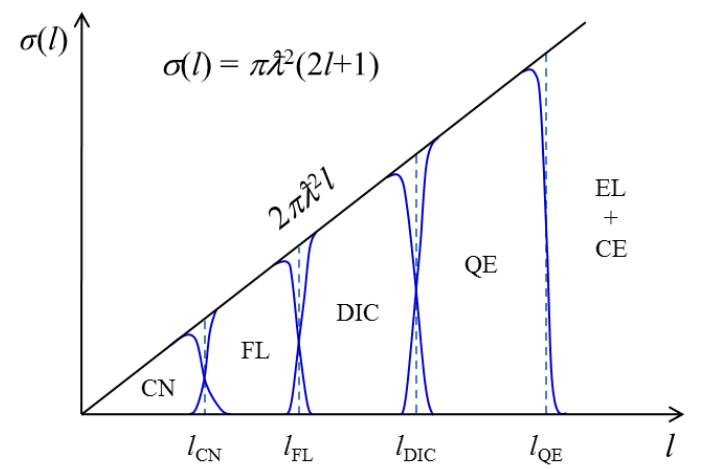
\includegraphics[width=0.6\textwidth]{lcn}
    \bicaption{lcn示意图}{Schematic diagram of lcn}
    \label{fig:lcn}
\end{figure}

\textbf{参数说明：}

\begin{compactitem}
    \item \verb|[htbp]|：位置选项，依次尝试当前位置（h）、页面顶部（t）、底部（b）、单独页面（p）。
    \item \verb|\centering|：图片居中。
    \item \verb|width=0.6\textwidth|：图片宽度为版心宽度的60\%，可按需调整。
    \item \verb|\bicaption{中文}{英文}|：本模板要求中英双语图题（格式规范要求）。
    \item \verb|\label{fig:示例}|：标签，用于 \verb|\ref{fig:示例}| 引用。
\end{compactitem}

\textbf{图片格式建议：}
\begin{compactitem}
    \item 矢量图（折线图、柱状图等）：优先使用 \texttt{.pdf} 或 \texttt{.eps}，缩放不失真。
    \item 位图（照片、实验截图）：使用 \texttt{.png}（无损）或 \texttt{.jpg}，分辨率建议 $\geq$ 300 DPI。
    \item 文件名不含中文和空格，如 \texttt{detector\_setup.pdf}。
    \item 所有图片放在 \texttt{figures/} 目录下，引用时只写文件名，不写路径和扩展名。
\end{compactitem}

\subsection{调整图片大小}

\begin{verbatim}
\includegraphics[width=0.8\textwidth]{图片名}    % 按版心宽度比例
\includegraphics[height=5cm]{图片名}             % 按固定高度
\includegraphics[scale=0.5]{图片名}              % 按缩放比例
\end{verbatim}

\subsection{图的引用规范}

正文中必须有对图的提示，引用方式：

\begin{verbatim}
如图~\ref{fig:detector}~所示，探测器由三层构成。
图~\ref{fig:spectrum}~为实验测量的能谱。
\end{verbatim}

\section{三线表（推荐格式）}

格式规范推荐使用三线表：只有顶线、栏目线和底线，无竖线。
使用 \texttt{booktabs} 宏包提供的命令（已包含在模板中）：

\begin{verbatim}
\begin{table}[H]
\centering
\bicaption{表题中文}{Table caption in English}
\label{tab:示例}
\begin{tabular}{lccc}
\toprule                              % 顶线（粗）
列标题1 & 列标题2 & 列标题3 & 列标题4 \\
\midrule                              % 栏目线（细）
数据1   & 数据2   & 数据3   & 数据4   \\
数据5   & 数据6   & 数据7   & 数据8   \\
\bottomrule                           % 底线（粗）
\end{tabular}
\end{table}
\end{verbatim}

示例——实验参数表：

\begin{table}[H]
\centering
\bicaption{实验束流参数}{Beam parameters of the experiment}
\label{tab:beam}
\begin{tabular}{lcc}
\toprule
参数 & 数值 & 单位 \\
\midrule
束流能量 & 100 & MeV \\
束流强度 & $1 \times 10^6$ & pps \\
靶厚 & 2.0 & mg/cm$^2$ \\
探测角度 & 15--150 & 度 \\
\bottomrule
\end{tabular}
\end{table}

如表~\ref{tab:beam}~所示，束流能量为100 MeV。

\textbf{列格式说明（tabular参数）：}
\begin{compactitem}
    \item \texttt{l}：左对齐；\texttt{c}：居中；\texttt{r}：右对齐
    \item \texttt{p\{3cm\}}：固定宽度列，超出自动换行
    \item 竖线 \verb+|+ 可加列分隔线（三线表不使用）
\end{compactitem}

\section{带脚注的表格}

对表中数据需要补充说明时，使用 \texttt{threeparttable} 环境：

\begin{verbatim}
\begin{table}[H]
\centering
\bicaption{带脚注的表格示例}{Table with footnotes}
\begin{threeparttable}
\begin{tabular}{lcc}
\toprule
方法 & $\beta_3$ & $\delta_3$ (fm) \\
\midrule
电子散射\tnote{$a$} & 0.120 & 0.85 \\
$\alpha$散射\tnote{$b$}  & 0.118 & 0.84 \\
\bottomrule
\end{tabular}
\begin{tablenotes}
    \item[$a$] 束流能量75 MeV。
    \item[$b$] 束流能量79.1 MeV。
\end{tablenotes}
\end{threeparttable}
\end{table}
\end{verbatim}

\begin{table}[H]
\centering
\bicaption{$^{208}$Pb 形变参数的不同测量方法对比}{Comparison of $^{208}$Pb deformation parameters from different methods}
\begin{threeparttable}
\begin{tabular}{lcc}
\toprule
方法 & $\beta_3$ & $\delta_3$ (fm) \\
\midrule
电子散射\tnote{$a$} & 0.120 & 0.85 \\
$\alpha$散射\tnote{$b$} & 0.118 & 0.84 \\
\bottomrule
\end{tabular}
\begin{tablenotes}
    \item[$a$] 束流能量75 MeV。
    \item[$b$] 束流能量79.1 MeV。
\end{tablenotes}
\end{threeparttable}
\end{table}

\section{合并单元格}

使用 \verb|\multicolumn| 合并横向单元格，\verb|\multirow| 合并纵向单元格（需要 \texttt{multirow} 宏包）：

\begin{verbatim}
\multicolumn{列数}{对齐}{内容}    % 横向合并
\multirow{行数}{宽度}{内容}      % 纵向合并（需 \usepackage{multirow}）
\end{verbatim}

\section{图表的跨页处理}

当表格过长需要跨页，使用 \texttt{longtable} 环境：

\begin{verbatim}
\begin{longtable}{lcc}
\caption{跨页长表格}\label{tab:long} \\
\toprule
列1 & 列2 & 列3 \\
\midrule
\endfirsthead
% 续页表头（格式规范要求续表重复表头）
\multicolumn{3}{l}{\tablename~\thetable（续）} \\
\toprule
列1 & 列2 & 列3 \\
\midrule
\endhead
\bottomrule
\endfoot
% 表格内容行
数据1 & 数据2 & 数据3 \\
% ... 更多行
\end{longtable}
\end{verbatim}

\section{分图}

含有分图时，分图题置于各分图之下，分图号用 a)、b) 表示，整图标题置于所有分图之后。
使用 \texttt{subcaption} + \texttt{bicaption} 宏包（已在模板中载入），分图题支持中英双语：

\begin{verbatim}
\begin{figure}[htbp]
    \centering
    \begin{subfigure}{0.45\textwidth}
        \centering
        \includegraphics[width=\textwidth]{图1}
        \bisubcaption{中文分图题a}{English subcaption a}
        \label{fig:sub-a}
    \end{subfigure}
    \hfill
    \begin{subfigure}{0.45\textwidth}
        \centering
        \includegraphics[width=\textwidth]{图2}
        \bisubcaption{中文分图题b}{English subcaption b}
        \label{fig:sub-b}
    \end{subfigure}
    \bicaption{整图中文标题}{Overall English caption}
    \label{fig:subfig}
\end{figure}
\end{verbatim}

实际效果如图~\ref{fig:subfig-example}~所示：

\begin{figure}[htbp]
    \centering
    \begin{subfigure}{0.45\textwidth}
        \centering
        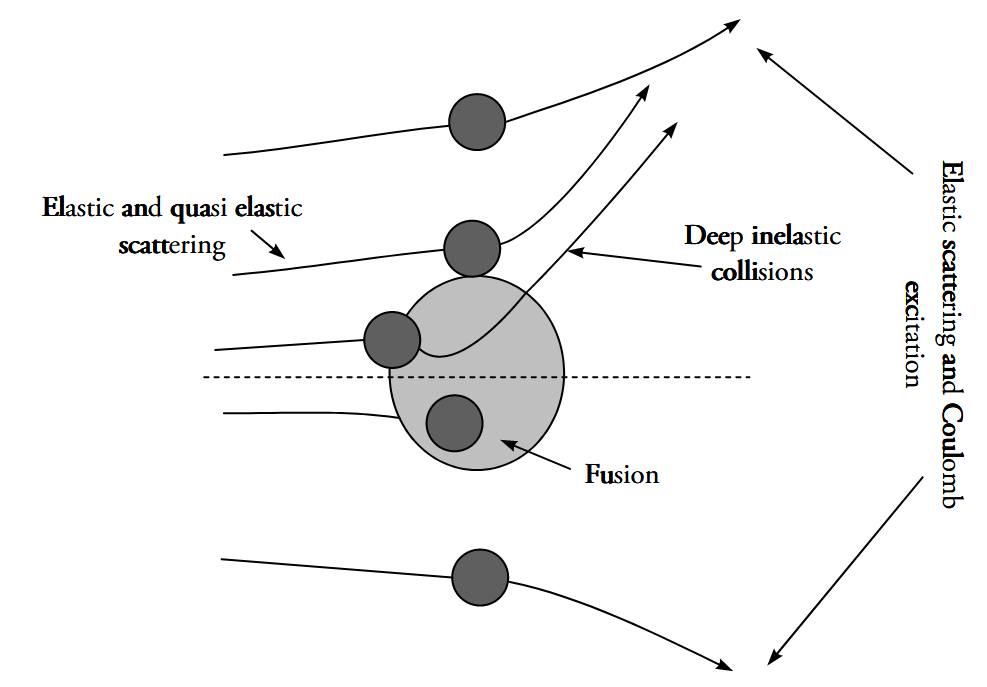
\includegraphics[width=\textwidth]{ion}
        \bisubcaption{离子示意图}{Schematic diagram of ions}
        \label{fig:sub-ion}
    \end{subfigure}
    \hfill
    \begin{subfigure}{0.45\textwidth}
        \centering
        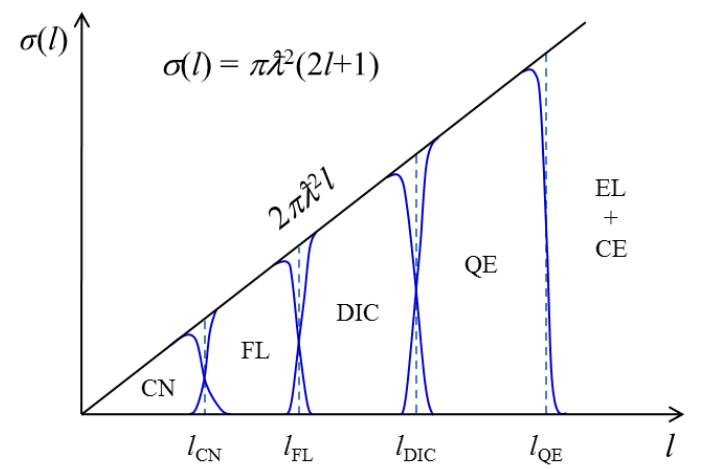
\includegraphics[width=\textwidth]{lcn}
        \bisubcaption{lcn示意图}{Schematic diagram of lcn}
        \label{fig:sub-lcn}
    \end{subfigure}
    \bicaption{分图示例}{Example of subfigures}
    \label{fig:subfig-example}
\end{figure}

\section{本章小结}

本章介绍了图片插入、三线表制作、带脚注表格、合并单元格、
跨页表格以及分图的使用方法。
第~\ref{chap:references}~章将介绍参考文献的管理与引用。
   % 第四章：图片与表格
%%% Local Variables:
%%% mode: latex
%%% TeX-master: t
%%% End:

% ============================================================
% 第五章：参考文献
% 本章介绍 BibTeX 文献管理和引用方法。
% ============================================================

\chapter{参考文献}\label{chap:references}

\section{参考文献格式规范}

本院格式规范要求：
\begin{compactitem}
    \item 参考文献按在正文中出现的顺序编号，如 \cite{MARTIN20131497}。
    \item 引用标号置于所引内容最后一个字右上角。
    \item 所有被引用文献必须列入参考文献，同一篇文献只用一个序号。
    \item 参考文献内容使用小四号宋体，1.25倍行距。
\end{compactitem}

\section{BibTeX 文件格式}

参考文献存放在 \texttt{bib/refs.bib} 文件中，每条文献是一个条目，格式如下：

\subsection{期刊论文（article）}

\begin{verbatim}
@article{引用key,
    author  = {作者1 and 作者2 and 作者3},
    title   = {论文题目},
    journal = {期刊名},
    year    = {2023},
    volume  = {100},
    number  = {1},
    pages   = {1--10},
    doi     = {10.xxxx/xxxxx}
}
\end{verbatim}

示例（本模板 \texttt{bib/refs.bib} 中已有的条目）：
\begin{verbatim}
@article{MARTIN20131497,
    author  = {M.J. Martin},
    title   = {Nuclear Data Sheets for A = 152},
    journal = {Nuclear Data Sheets},
    year    = {2013},
    volume  = {114},
    pages   = {1497--1847}
}
\end{verbatim}

\subsection{学位论文（phdthesis / mastersthesis）}

\begin{verbatim}
@phdthesis{张三2023,
    author = {张三},
    title  = {基于XXXX方法的核反应截面研究},
    school = {中国原子能科学研究院},
    year   = {2023},
    type   = {博士学位论文}
}

@mastersthesis{李四2022,
    author = {李四},
    title  = {XXX实验方案设计},
    school = {中国原子能科学研究院},
    year   = {2022}
}
\end{verbatim}

\subsection{书籍（book）}

\begin{verbatim}
@book{Blatt1952,
    author    = {Blatt, John M. and Weisskopf, Victor F.},
    title     = {Theoretical Nuclear Physics},
    publisher = {Springer},
    address   = {New York},
    year      = {1952}
}
\end{verbatim}

\subsection{会议论文（inproceedings）}

\begin{verbatim}
@inproceedings{Wang2022,
    author    = {Wang, X. and Zhang, Y.},
    title     = {Title of the Paper},
    booktitle = {Proceedings of the International Conference on ...},
    year      = {2022},
    pages     = {100--105}
}
\end{verbatim}

\section{引用命令}

本模板提供两种引用命令，对应院格式规范中的两种标注方式：

\begin{compactitem}
    \item \verb|\cite{key}|：行内引用，编号以方括号形式嵌入正文，
          效果如 \cite{KIBEDI200235}，适合"由文献[X]可知……"的写法。
    \item \verb|\upcite{key}|：上标引用，编号以上标方括号形式出现，
          效果如\upcite{MARTIN20131497}，适合在句末或词后标注，
          是本院格式规范中最常用的引用形式。
\end{compactitem}

\verb|\upcite| 是本模板在 \texttt{main.tex} 中自定义的命令：
\begin{verbatim}
\newcommand{\upcite}[1]{\textsuperscript{\textsuperscript{\cite{#1}}}}
\end{verbatim}

引用多篇文献时，用英文逗号分隔多个 key，编号将自动合并：
\begin{verbatim}
\cite{key1,key2,key3}      % 行内，效果：[1,2,3]
\upcite{key1,key2,key3}    % 上标，效果：[1,2,3]（上标）
\end{verbatim}
实际效果：\cite{MARTIN20131497,KIBEDI200235}（行内）；\upcite{MARTIN20131497,KIBEDI200235}（上标）。

格式规范示例：

\begin{verbatim}
% 上标引用（推荐，句末标注）
二次铣削\upcite{ref1}可以显著提高表面质量。
原位生成的TiB主要有针状或晶须状\upcite{ref2,ref3}。

% 行内引用（用于"由文献[X]可知"句式）
由文献\cite{ref4,ref5}可知，蠕变断裂以沿晶断裂为主。
\end{verbatim}

\section{如何获取 BibTeX 条目}

不需要手动输入每条文献，可以从数据库直接导出：

\subsection{从 Google Scholar 导出}

\begin{compactenum}
    \item 搜索文献，点击文献下方的引号图标（引用）。
    \item 在弹出窗口底部点击"BibTeX"。
    \item 复制全部内容，粘贴到 \texttt{bib/refs.bib} 文件中。
\end{compactenum}

\subsection{从 CNKI（知网）导出}

\begin{compactenum}
    \item 搜索文献，勾选需要的文献。
    \item 点击"导出与分析" → "导出文献"。
    \item 选择"BibTeX"格式，下载并合并到 \texttt{refs.bib}。
\end{compactenum}

\subsection{从 Web of Science / Scopus 导出}

\begin{compactenum}
    \item 选中文献，点击"导出"（Export）。
    \item 选择"BibTeX"格式并下载。
\end{compactenum}

\subsection{使用 JabRef 管理文献}

JabRef 是一款开源的 BibTeX 文献管理工具，可图形化管理 \texttt{.bib} 文件，
支持从 DOI、arXiv、ISBN 自动填充文献信息，强烈推荐使用。

\section{引用 key 的命名建议}

BibTeX 的 key（如 \texttt{MARTIN20131497}）用于在正文中引用，
建议采用统一的命名规则：

\begin{compactitem}
    \item 英文文献：\texttt{作者姓+年份}，如 \texttt{Blatt1952}
    \item 中文文献：\texttt{作者姓+年份}，如 \texttt{张三2023}
    \item 同一作者同一年多篇：加字母区分，如 \texttt{Wang2022a}、\texttt{Wang2022b}
\end{compactitem}

\textbf{注意}：key 不能含有中文，不能含有空格，区分大小写。

\section{参考文献样式}

本模板默认使用 GB/T 7714 顺序编码制（数字引用）：

\begin{verbatim}
% main.tex 中的设置（默认）
\bibliographystyle{gbt7714-numerical}
\bibliography{bib/refs}
\end{verbatim}

如需切换为著者-出版年制（如"[张三, 2023]"形式），修改为：

\begin{verbatim}
\bibliographystyle{ustcauthoryear}
\end{verbatim}

\section{本章小结}

本章介绍了 BibTeX 文件的格式、各类文献的写法、引用命令的使用，
以及从主流数据库导出文献条目的方法。
第~\ref{chap:advanced}~章将介绍代码块、算法和其他高级排版功能。
   % 第五章：参考文献
%%% Local Variables:
%%% mode: latex
%%% TeX-master: t
%%% End:

% ============================================================
% 第六章：高级功能
% 本章介绍代码块、算法伪代码、附录，以及常见错误解决方法。
% ============================================================

\chapter{高级功能}\label{chap:advanced}

\section{代码块}

使用 \texttt{listings} 宏包插入带语法高亮的代码，该宏包已包含在模板中。

\subsection{行内代码}

短代码片段可用 \verb|\verb| 命令：
\begin{verbatim}
使用 \verb|\cite{key}| 引用文献。
\end{verbatim}

\subsection{代码块环境}

较长的代码使用 \texttt{lstlisting} 环境：

\begin{verbatim}
\begin{lstlisting}[language=Python, caption={数据处理脚本}]
import numpy as np
import matplotlib.pyplot as plt

data = np.loadtxt('spectrum.dat')
energy = data[:, 0]
counts = data[:, 1]

plt.plot(energy, counts)
plt.xlabel('Energy (MeV)')
plt.ylabel('Counts')
plt.savefig('spectrum.pdf')
\end{lstlisting}
\end{verbatim}

效果：

\begin{lstlisting}[language=Python, caption={能谱数据处理脚本示例}]
import numpy as np
import matplotlib.pyplot as plt

data = np.loadtxt('spectrum.dat')
energy = data[:, 0]
counts = data[:, 1]

plt.plot(energy, counts)
plt.xlabel('Energy (MeV)')
plt.ylabel('Counts')
plt.savefig('spectrum.pdf')
\end{lstlisting}

支持的语言包括：\texttt{Python}、\texttt{C}、\texttt{C++}、\texttt{Fortran}、
\texttt{Matlab}、\texttt{bash} 等。

\subsection{从文件插入代码}

如果代码较长，可以直接读取外部文件：

\begin{verbatim}
\lstinputlisting[language=C++,
    caption={主程序}]{code/main.cpp}
\end{verbatim}

\section{算法伪代码}

使用 \texttt{algorithm2e} 环境排版算法伪代码，该宏包已包含在模板中。

\begin{verbatim}
\begin{algorithm}[H]
\caption{蒙特卡洛模拟算法}
\SetAlgoLined
初始化粒子位置和动量\;
\While{未达到收敛条件}{
    随机抽样粒子初始状态\;
    \For{每个粒子}{
        跟踪粒子在介质中的传输\;
        记录能量沉积\;
    }
    统计能谱分布\;
}
输出模拟结果\;
\end{algorithm}
\end{verbatim}

效果：

\normalem
\begin{algorithm}[H]
\caption{蒙特卡洛模拟算法}
\SetAlgoLined
初始化粒子位置和动量\;
\While{未达到收敛条件}{
    随机抽样粒子初始状态\;
    \For{每个粒子}{
        跟踪粒子在介质中的传输\;
        记录能量沉积\;
    }
    统计能谱分布\;
}
输出模拟结果\;
\end{algorithm}
\ULforem

常用算法命令：
\begin{compactitem}
    \item \verb|\While{条件}{内容}|：while 循环
    \item \verb|\For{条件}{内容}|：for 循环
    \item \verb|\If{条件}{内容}|：if 语句
    \item \verb|\eIf{条件}{then}{else}|：if-else 语句
    \item \verb|\KwIn{输入}|、\verb|\KwOut{输出}|：输入输出说明
    \item 行末加 \verb|\;|：表示语句结束（显示分号）
\end{compactitem}

\section{附录}

附录适合放置篇幅较大的推导过程、原始数据、程序源码等内容，
正文中不必展开但有参考价值的材料。

在 \texttt{main.tex} 中取消附录的注释：
\begin{verbatim}
\backmatter
\appendix
\chapter{附录}

附录      % 取消此行注释以启用附录
\input{chapters/acknowledgements}
\end{verbatim}

在 \texttt{chapters/appendix.tex} 中写附录内容：
\begin{verbatim}
\chapter{附录标题}\label{app:label}

附录中的图表公式另编排序号，如 A.1, A.2...
与正文分开编号，自动处理。
\end{verbatim}

\section{物理量和单位}

核物理论文中常用的特殊写法：

\begin{compactitem}
    \item 核素符号：\verb|$^{208}$Pb| → $^{208}$Pb；\verb|$^{16}$O| → $^{16}$O
    \item 能量单位：MeV、MeV/$c^2$（质量）、MeV/$c$（动量）
    \item 截面单位：\verb|mb（毫靶）| 或 \verb|fm$^2$|；$1$ b $= 10^{-24}$ cm$^2$
    \item 运动量符号：\verb|$Q$值|、\verb|$\sigma$截面|（需要在公式中定义）
    \item 数量级：\verb|$1.5 \times 10^{-3}$| → $1.5 \times 10^{-3}$（不用 E-3）
\end{compactitem}

\section{常见编译错误及解决方法}

\subsection{undefined control sequence（未定义命令）}

\textbf{原因}：使用了未加载的宏包中的命令，或命令拼写有误。

\textbf{解决}：检查命令拼写；确认相关宏包已在 \texttt{main.tex} 或 \texttt{ustcextra.sty} 中加载。

\subsection{Overfull \\hbox（行超出版心）}

\textbf{原因}：某段文字或公式太长，\LaTeX{} 无法正常断行。

\textbf{解决}：
\begin{compactitem}
    \item 在超长英文单词中手动添加断词提示：\verb|\-|，如 \verb|super\-con\-duc\-tor|
    \item 表格列宽过窄时改用 \texttt{p\{宽度\}} 列格式
    \item 长公式使用 \texttt{align} 环境换行
\end{compactitem}

\subsection{参考文献不显示 / 显示 [?]}

\textbf{原因}：未运行 BibTeX，或 key 不匹配。

\textbf{解决}：
\begin{compactenum}
    \item 确认已按顺序运行：\texttt{xelatex → bibtex → xelatex → xelatex}
    \item 检查 \texttt{bib/refs.bib} 中的 key 与 \verb|\cite{key}| 完全一致（区分大小写）
    \item 确认 \texttt{main.tex} 中 \verb|\bibliography{bib/refs}| 路径正确
\end{compactenum}

\subsection{图片未找到}

\textbf{原因}：文件路径或文件名有误。

\textbf{解决}：
\begin{compactitem}
    \item 确认图片在 \texttt{figures/} 目录下
    \item 文件名不含中文和空格
    \item 在 \verb|\includegraphics{文件名}| 中只写文件名，不写 \texttt{figures/} 前缀（已在 \texttt{main.tex} 中通过 \verb|\graphicspath| 配置）
\end{compactitem}

\subsection{字体警告 / 找不到字体}

\textbf{原因}：系统中缺少所需中文字体。

\textbf{解决}：确保 \texttt{main.tex} 文档类选项中有 \texttt{AutoFakeFont=true}（默认已添加），
该选项在缺少字体时自动合成加粗/斜体，避免报错。

\section{有用的写作技巧}

\begin{compactitem}
    \item \textbf{快速查找符号}：访问 \texttt{detexify.kirelabs.org}，手写符号即可识别对应命令。
    \item \textbf{段落过长警告}：编译时出现 \texttt{Underfull \\hbox} 通常无害，可忽略。
    \item \textbf{保持源码整洁}：每个句子单独一行，便于 Git 追踪修改和与导师协作。
    \item \textbf{备份}：推荐用 Git 管理论文版本，每次重大修改提交一次，永远不会丢失。
\end{compactitem}

\section{本章小结}

本章介绍了代码块、算法伪代码、附录的使用方法，
以及核物理论文中常用的符号写法和常见编译错误的解决方案。
至此，本使用说明涵盖了论文写作的主要排版功能。

在正式撰写论文时，请将各章节中的说明性内容替换为你自己的研究内容。
如有疑问，可参考 \texttt{README.md} 中的常见问题部分，
或查阅《\LaTeX{} 入门》（lshort-zh-cn）文档。
   % 第六章：高级功能
% \input{chapters/chap07} % 如需更多章节，取消注释并新建对应文件

\bibliographystyle{gbt7714-numerical}  % 参考文献格式
\bibliography{bib/refs}                % 参考文献数据库文件

\backmatter
\appendix
\chapter{附录}

附录      % 附录（如无，注释该行）
\input{chapters/acknowledgements}  % 致谢
\begin{publications}

% 发表论文列表

\begin{enumerate}
    \renewcommand{\labelenumi}{[\theenumi].}
    \item XXX, XXX, XXX, et.al. EXXXXXX[J].  XXXXX,202X.(accepted);
\end{enumerate}


\end{publications}
      % 发表论文列表

\end{document}
